\documentclass[11pt,a4paper,fleqn]{article}

\usepackage[top=2.54cm, bottom=2.54cm, left=3.18cm, right=3.18cm]{geometry}
\usepackage[pdftex]{graphicx}
\usepackage{amsmath, amsthm, amssymb}
\usepackage{setspace}
\usepackage{mdwlist}
\usepackage{newclude}
\usepackage{enumerate}
\usepackage{array}
\usepackage{bussproofs}
\usepackage{lastpage}
\usepackage{hyperref}
\usepackage{fancyhdr}
\usepackage[normalem]{ulem}
\usepackage{longtable}

\pagestyle{fancy}
%\fancyhf{}

\onehalfspace

\theoremstyle{definition}
\newtheorem{definition}{Definition}[subsection]

\theoremstyle{plain}
\newtheorem{theorem}[definition]{Theorem}

\theoremstyle{plain}
\newtheorem{lemma}[definition]{Lemma}

\theoremstyle{definition}
\newtheorem{proposition}[definition]{Proposition}

\setlength{\mathindent}{0pt}

\renewcommand{\thefigure}{\thesection.\arabic{figure}}

\newenvironment{myitemize}
{\begin{list}{$ \bullet $}{
  \topsep=2pt
  \itemsep=2pt
  \parsep=0pt
  \parskip=0pt
  \labelsep=5pt
  \labelwidth=20pt}}
{\end{list}}

\newcommand{\litp}{[\![}
\newcommand{\ritp}{]\!]}
\newcommand{\eqnline}{\\[5pt]}

\newcommand{\tc}{\mathord{:}}
\newcommand{\ta}{\mathord{\to}}

\begin{document}

\begin{titlepage}
\begin{center}
% Upper part of the page

\includegraphics[width=0.2\textwidth]{./images/bham_logo}\\[1cm]
\textsc{\LARGE University of Birmingham}\\[0.5cm]
\textsc{\Large School of Computer Science}\\[1.5cm]
\textsc{\large Final Year Project}\\[0.3cm]
% Title
\rule{\linewidth}{0.5mm} \\[0.6cm]
{ \huge \bfseries The Curry-Howard Isomorphism}\\[0.1cm]
\rule{\linewidth}{0.5mm} \\[1.5cm]
% Author and supervisor
\begin{minipage}{0.4\textwidth}
\begin{flushleft} \large
\emph{Author:}\\
Chuangjie \textsc{Xu}
\end{flushleft}
\end{minipage}
\begin{minipage}{0.4\textwidth}
\begin{flushright} \large
\emph{Supervisor:} \\
Prof. Achim \textsc{Jung}
\end{flushright}
\end{minipage}
\vfill
% Bottom of the page
{\large \today}
\end{center}
\end{titlepage}

\pagenumbering{roman}
\cfoot{\thepage}
\begin{abstract}
\addcontentsline{toc}{section}{Abstract}
Systems of formal logic, as encountered in \emph{proof theory}, tightly correspond to computational calculi, as found in \emph{type theory}, which is known as the \emph{Curry-Howard Isomorphism}. This correspondence has been extended to cartesian closed categories, a special kind of categories in \emph{category theory}. This project focuses on this three-way correspondence and the ways in which they connect to each other. While the correspondence looks superficially straightforward, a considerable quantity of care has to be applied to prove it in full generality. Most of the proofs given in this dissertation are carried out by induction on derivations or terms. The main conclusions drawn from this study are that one can obtain a lambda term in simply typed lambda calculus from a proof in intuitionistic propositional logic, and vice versa. In addition, cartesian closed categories can be used as a framework for describing the denotational semantics of both the simply typed lambda calculus and intuitionistic propositional logic.\\[50pt]
\end{abstract}

\renewcommand{\abstractname}{Acknowledgements}
\begin{abstract}
\addcontentsline{toc}{section}{Acknowledgements}
I am sincerely indebted and grateful to Achim Jung, my supervisor, for his encouragement, guidance and kindness, for keeping this research-oriented project enjoyable, and for helping me develop an understanding in the subject of theoretical computer science.

My heartfelt gratitude also goes to Martin Escardo, for supervising my individual study project and organising the course of domain theory, both of which are greatly beneficial to this project as well as my preparation for further study in their research area.

Besides, I would like to thank the group of Mathematical Foundations of Computer Science, for giving mathematical lunch talks every week, which provides me a valuable opportunity to know what current researches the mathematicians and computer scientists in this department are doing.

Last but not least, words alone cannot express the gratitude I owe to my family, particularly to my parents, for the unconditional love and everything they have given me.
\end{abstract}


\newpage
\tableofcontents

\clearpage
\setcounter{page}{1}
\pagenumbering{arabic}
\cfoot{Page \thepage\ of \pageref{LastPage}}
\section{Introduction}
\label{sec:introduction}

Logicians must be familiar with modus ponens $ P\to Q,P\vdash Q $, a very common rule of inference, saying that given implication $ P\to Q $ and proposition $ P $, we have $ Q $. Programmers may frequently use function application: if $ f $ is a function of type $ P\to Q $ and $ x $ is an argument of type $ P $, then the application $ f x $ is of type $ Q $. Interestingly, modus ponens behaves the same as function application. So, are proofs related to programs? Yes, there is a precise correspondence between them which is described in the Curry-Howard Isomorphism.

In the 1930s, Haskell Curry observed a correspondence between types of combinators and propositions in intuitionist implicational logic. But, at that time, it was viewed as no more than a curiosity. About three decades later, William Howard extended this correspondence to first order logic by introducing dependent types. Therefore, this correspondence is called the Curry-Howard Isomorphism.

The Curry-Howard Isomorphism states a correspondence between systems of formal logic and computational calculi. For years, it has been extended to more expressive logics, e.g. higher order logic, and other mathematical systems, e.g. cartesian closed categories. In this project, I mainly probed into one of its extensions, the three-way-correspondence between intuitionistic propositional logic, simply-typed lambda calculus and cartesian closed categories, with propositions or types being interpreted as objects and proofs or terms as morphisms.

\begin{center}
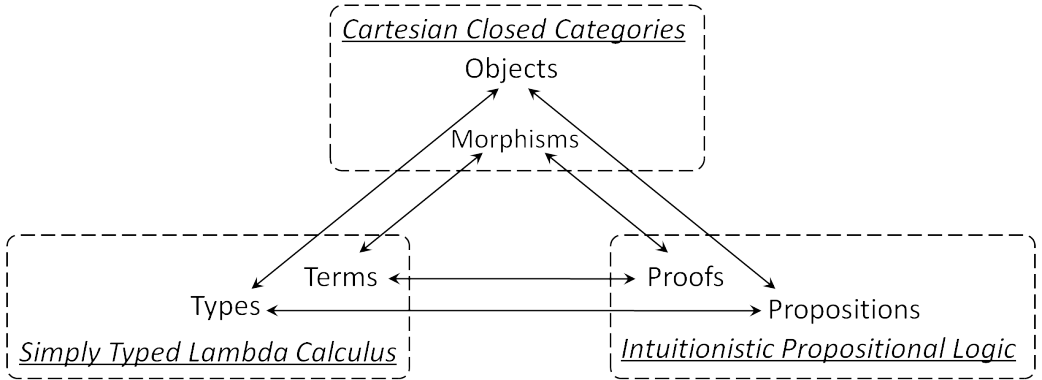
\includegraphics[width=0.9\textwidth]{./images/triangle}
\end{center}

Intuitionistic logic is a formalization of Brouwer’s intuitionism. As the founder of intuitionism, L. E. J. Brouwer avoided use of formal language or logic all his life. But his attitude did not stop others considering formalizations of parts of intuitionism. In the 1930s, Arend Heyting, a former student of Brouwer, produced the first complete axiomatizations for intuitionistic propositional and predicate logic. In intuitionistic logic, the law of excluded middle and double negation elimination are no longer axioms.

The lambda calculus was introduced by Alonzo Church in the early 1930s as a formal system to provide a functional foundation for mathematics. Since Church’s original system was shown to be logically inconsistent, he gave just a consistent subtheory of his original system dealing only with the functional part. Then, in 1940, Church also introduced a typed interpretation of the lambda calculus by giving each term a unique type. Today, the typed lambda calculus serves as the foundation of the modern type systems in computer science.

Category first appeared in Samuel Eilenberg and Saunders Mac Lane’s paper written in 1945. It was originally introduced to describe the passage from one type of mathematical structure to another. In recent decades, category theory has found use for computer science. For instant, it has a profound influence on the design of functional and imperative programming languages, e.g. Haskell and Agda.

Looking from the historical perspective, these three different systems seem to have different origins, not related to each other. However, Joachim Lambek showed in the early 1970s that cartesian closed categories provided a formal analogy between proofs in intuitionistic propositional logic and types in combinatory logic. As a result, some people may use Curry-Howard-Lambek Isomorphism to refer to this three-way-correspondence.

\newpage
\section{Background}
\include*{bg_il}
\include*{bg_lc}
\include*{bg_cat}

\newpage
\section{Correspondences}
\include*{co_t2p}
\include*{co_p2t}
\include*{co_t2m}

\section{Reflections}
Doing a dissertation-only project was the most challenging but ambitious decision that I have made during my life in the University of Birmingham. As an overseas student, writing (in English) is definitely the most painful part of this project.

Though the correspondence seems to be straightforward, one needs to be very careful in the proofs. As far as some details are concerned, some terms may not correspond to proofs very tightly. The following is such a counter example.
\begin{center}
\AxiomC{}
\UnaryInfC{$ x \tc \sigma \vdash x : \sigma $}
\RightLabel{($ add $)}
\UnaryInfC{$ x \tc \sigma , y \tc \sigma \vdash x : \sigma $}
\RightLabel{($ \to $I)}
\UnaryInfC{$ x \tc \sigma \vdash \lambda y \tc \sigma. x : \sigma \ta \sigma $}
\RightLabel{($ \to $I)}
\UnaryInfC{$ \vdash \lambda x \tc \sigma. \lambda y \tc \sigma. x : \sigma \ta (\sigma \ta \sigma) $}
\DisplayProof \hspace*{10pt} $ \Longrightarrow $ \hspace*{10pt}
\AxiomC{}
\UnaryInfC{$ \sigma \vdash \sigma $}
\RightLabel{($ add $)}
\UnaryInfC{$ \sigma , \sigma \vdash \sigma $}
\RightLabel{($ \to $I)}
\UnaryInfC{$ \sigma \vdash \sigma \to \sigma $}
\RightLabel{($ \to $I)}
\UnaryInfC{$ \vdash \sigma \to (\sigma \to \sigma) $}
\DisplayProof
\end{center}
We erase all the terms in the derivation of $ \lambda x \tc \sigma. \lambda y \tc \sigma. x : \sigma \ta (\sigma \ta \sigma) $. But the result does not look like a valid proof since the context, as a set, should not contain repeated propositions. One may want to adjust it to obtain a proof of ``$\sigma \to (\sigma \to \sigma)$''. However, we cannot rebuild the original term (or a term $ \alpha $-equivalent to the original one) from this proof.
\begin{center}
\AxiomC{}
\UnaryInfC{$ \sigma \vdash \sigma $}
\RightLabel{($ \to $I)}
\UnaryInfC{$ \vdash \sigma \to \sigma $}
\RightLabel{($ add $)}
\UnaryInfC{$ \sigma \vdash \sigma \to \sigma $}
\RightLabel{($ \to $I)}
\UnaryInfC{$ \vdash \sigma \to (\sigma \to \sigma) $}
\DisplayProof \hspace*{10pt} $ \Longrightarrow $ \hspace*{10pt}
\AxiomC{}
\UnaryInfC{$ x \tc \sigma \vdash x: \sigma $}
\RightLabel{($ \to $I)}
\UnaryInfC{$ \vdash \lambda x \tc \sigma . x : \sigma \ta \sigma $}
\RightLabel{($ add $)}
\UnaryInfC{$ y \tc \sigma \vdash \lambda x \tc \sigma . x : \sigma \ta \sigma $}
\RightLabel{($ \to $I)}
\UnaryInfC{$ \vdash \lambda y \tc \sigma . \lambda x \tc \sigma . x : \sigma \ta (\sigma \ta \sigma) $}
\DisplayProof
\end{center}
One of the solutions to this problem is linear logic which is proposed as a refinement of classical and intuitionistic logic. But linear logic is not involved in this project.

During this project, most of the time was spent in learning foundations of category theory. It was difficult to show that \textsc{Pos}$_{\bot !}$ (the category of posets with bottom preserving maps given in section \ref{sec:bg_cat_ccc}) is not cartesian closed. Even though the supervisor allowed me to leave this tough question, I kept trying to solve it for several weeks. However, I was just able to show that the exponentials from \textsc{Pos} are not categorical exponentials in \textsc{Pos}$_{\bot !}$. Finally, this question was overcome under the guidance of the supervisor.

The literature \cite{AL91,BW95,LS86,Mit96} I have read, interprets $ \lambda^{unit,\times,\to} $ terms in cartesian closed categories and shows the cartesian closed structure of the category generated from $ \lambda^{unit,\times,\to} $. As discussed at the beginning of section \ref{sec:co_t2m}, their connection seems to be obvious. People are much more interested in revealing the obscure connection; therefore, with the advice of the supervisor, it was decided to prove the correspondence between $ \lambda^{\to} $ and CCCs, which is the main part of this project as well as my own contribution to this project.

Cartesian closed categories have several properties of importance, i.e. some special equations which hold in every CCC. Most categorical literature utilises diagrams to give proofs to these equations. However, beginners may find it difficult to see equations through diagrams. This dissertation provides both diagram-based and equation-based proofs to the equations. Both ways have their pros and cons. Given a complicated equation, its corresponding diagram may be too large to draw on an A4 paper. The equational ones provide proof step by step, which always makes the proof tedious and hard to remember. What is a good way to present proofs? This is another tough question I faced in this project.

All in all, it is really enjoyable to be immersed in this research-oriented project. For one thing, it increased my thirst for knowledge in theoretical computer science as well as improved my skills in research. For another, the connection between proof theory, type theory and category theory did amaze me. When looking at different mathematical subjects, I keep asking myself whether they can be linked to each other.


\newpage
\bibliographystyle{abbrv}
\bibliography{myref}
\nocite{*}
\addcontentsline{toc}{section}{References}

\end{document}
